\subsection{Cluster tests}\label{sec:clustertest}
In this section are the tests that requires the cluster. This is due to the size of the tests, and the expected time frame.
\todo{skriv mere}
\subsubsection{Feature tests}\label{sec:feattest}
Some features might be more expressive than others, and finding the set of features that will yield the best result is imperative. The tests on the cluster are performed with logistic regression using stochastic gradient descent and L2 regularization with a ridge value of 0.01. 
For each feature test 1348428 games are used for training and 577552 games are used for evaluation. 
The different feature sets tested are:
\begin{enumerate}
\item Singles
\item Pairs
\item Singles, pairs
\item Singles, pairs, counters 
\item Singles, pairs, counters, best-ranks
\item All prematch: Singles, pairs, counters, best-ranks, runes, lanes, queue, spells
\end{enumerate}


\begin{figure}[!htb]
  \centering
  % Graph for feature tests. 
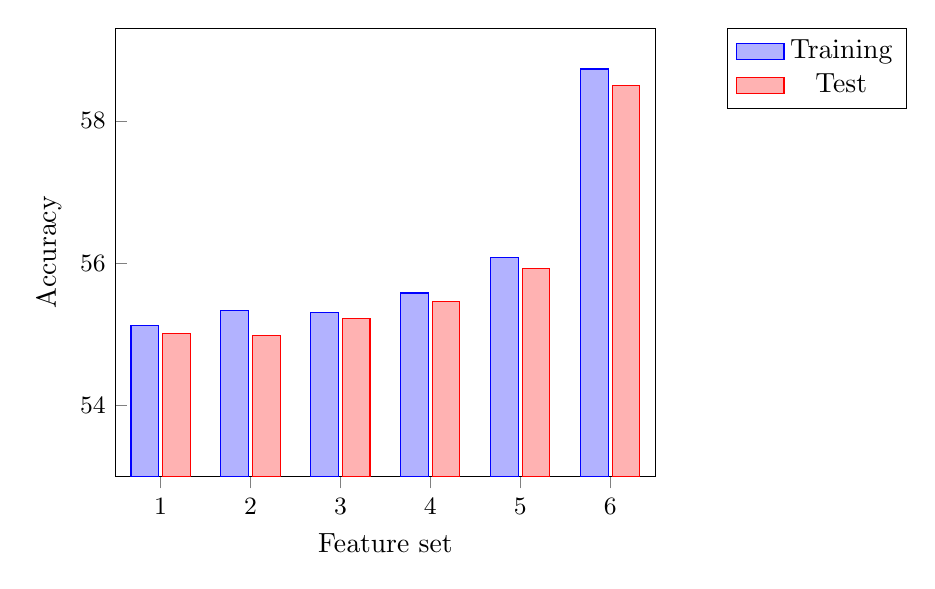
\begin{tikzpicture}
\begin{axis}[
    ybar,
    ylabel = Accuracy,
    xlabel = Feature set,
    tick label style={font=\small},
    tickpos=left,
    xticklabels={1, 2, 3, 4, 5, 6}, 
    xtick={1,2,3,4,5, 6},
    ymin=53,
    legend entries={Training,Test},
    legend style={at={(1.3,1.0)},
        anchor=north,legend columns=1
    },
    legend image code/.code={%
      \draw[#1] (0cm,-0.1cm) rectangle (0.6cm,0.1cm);
    }   
    ]   
    \addplot +[bar shift=-.2cm] coordinates {(1,55.12) (2,55.34) (3,55.31)  (4,55.58)     (5,56.08)  (6, 58.73)};

    \addplot  +[bar shift=.2cm]coordinates {(1,55.01) (2,54.98) (3,55.22) (4,  55.46) (5,55.92) (6, 58.50)};

\end{axis}
\end{tikzpicture}
   \caption{Accuracy of features}\label{fig:cluster-feat}
\end{figure}

The feature evaluation results from \Cref{fig:cluster-feat} shows two interesting results, by looking at each individual test case we see the we have almost no overfitting. The largest difference is data point 2: (pairs) with a difference of $3.610^{-3}$ percentage points. The results shows some tendency between the complexity of the model and the performance of the classifier. Higher complexity in general yields a better classifier. The best result was achieved using all pre-match features.




